\chapter{Commande proportionnelle intégrale à 6 DOF}
\minitoc
\label{chap:6DOF}

\section{Motivation}
\label{sec:motivation6DOF}
Nous avons observé expérimentalement dans le chapitre \ref{chap:3DOF} qu'un drone \textit{tailsitter} pouvez se stabiliser en stationnaire face à du vent vers les points d'équilibre décrit dans la section \ref{sec:eq_vent} grâce à une architecture de commande linaire. Cette dernière est basée sur un retour de sortie, proportionnel intégral, libérant deux degrés de liberté sur l'orientation du drone 


\section{Schéma de commande linéaire proportionnel intégral : 6 Dof}
\label{sec:6dofcmd}
\subsection{Description du schéma de contrôle}
\label{sec:ctl_sche}

Une inspection minutieuse des matrices de commande et d'entrée des perturbations $\boldsymbol{G}_{w}$ et $\boldsymbol{E}_{w}$ du modèle \eqref{eq:lpv_linearisation} (voir la sortie de l'Algorithme~\ref{alg:linea}) suggère une architecture de contrôle efficace pour rejeter une perturbation de vent constante $\boldsymbol{w}$. En effet, les ailerons et les hélices peuvent être utilisés symétriquement pour générer respectivement un moment autour de l'axe $y_{[\text{b}]}$, vérifiant l'équation \eqref{eq:momenty} et une force le long de l'axe $x_{[\text{b}]}$, vérifiant l'équation \eqref{eq:forcex}, compensant ainsi l'effet de la perturbation. Néanmoins, il reste une force le long de l'axe $z_{[\text{b}]}$ à compenser en vérifiant l'équation \eqref{eq:forcez}, et une action intégrale peut converger asymptotiquement vers la force désirée, même avec une perturbation du vent non mesurée $\boldsymbol{w}$. Nous pouvons donc stabiliser le drone à l'équilibre en vol stationnaire tel que caractérisé dans le Théorème~\ref{thm:eqs}. Comme nous ne mesurons pas le vent $\boldsymbol{w}$, les valeurs de $\psi$ et $\theta$ dans l'Algorithme~\ref{alg:eq} sont inconnues. Le contrôleur proposé, illustré à la Fig.~\ref{fig:commande_int6DOF}, utilise l'action intégrale pour faire converger ces angles vers leur valeur d'équilibre. Le bouclage utilise les variables d'erreur suivante : 
\begin{align}
    \boldsymbol{e}_{p}= \boldsymbol{r}_{p} - \boldsymbol{p}, \; \boldsymbol{e}_{v \epsilon \omega} = -  
       \left[ \begin{smallmatrix} \mathbb{I}_{3}  & \mathbb{0}_{3\times 1} & \mathbb{0}_{3\times 2} & \mathbb{0}_{3}\\
       \mathbb{0}_{1\times 3}  & 1 & \mathbb{0}_{1\times 2} & \mathbb{0}_{1 \times 3} \\
           \mathbb{0}_{3}  & \mathbb{0}_{3\times 1} & \mathbb{0}_{3\times 2} &   \mathbb{I}_{3}
           \end{smallmatrix} \right]
    \smallmat{
           \tilde{\boldsymbol{v}} \\
           \tilde{\boldsymbol{\epsilon}} \\
           \tilde{\boldsymbol{\omega}}_{\text{b}} 
    }.
  \label{eq:error_var}
  \end{align} 
Elles doivent converger vers zéro dans le cas de vol stationnaire et pour n'importe quelle position de référence constante $\boldsymbol{r}_{p} \in \mathbb{R}^{3}$. Notons que $\boldsymbol{r}_{p}$ est l'entrée de référence du schéma de contrôle.

Les variables d'erreur dans \eqref{eq:error_var} peuvent être représentées comme dans le schéma  de la Fig.~\ref{fig:commande_int6DOF} en définissant la sortie $\boldsymbol{y}\in \real^{10}$ de la dynamique du système linéarisée \eqref{eq:lpv_linearisation}, ayant le vecteur d'état incrémental $\boldsymbol{\tilde{x}} \in \real^{10 \times 1}$ défini ci-dessous : 
\begin{align}
    \label{eq:output_lin}
    \boldsymbol{y} = \boldsymbol{C} \boldsymbol{\tilde{x}} + \smallmat{\boldsymbol{p}_{\mathrm{eq}} \\ \mathbb{0}_{7 \times 1}}, \quad
 \boldsymbol{C} := \smallmat{\mathbb{I}_{6} & \mathbb{0}_{6\times 1} & \mathbb{0}_{6\times 2} &\mathbb{0}_{6\times 3}\\
    \mathbb{0}_{1\times 6} & 1 & \mathbb{0}_{1\times 2} &\mathbb{0}_{1\times 3}\\
    \mathbb{0}_{3\times 6} & \mathbb{0}_{3\times 1} & \mathbb{0}_{3\times 2} &  \mathbb{I}_{3}
},
\end{align}
où la matrice de sortie $\boldsymbol{C} \in \real^{10\times12}$ enlève la composante $\tilde{\epsilon}_{2}$ et $\tilde{\epsilon}_{3}$ du vecteur d'état $\tilde{\boldsymbol{x}}$. 

\begin{figure}[t!]
    \centering
    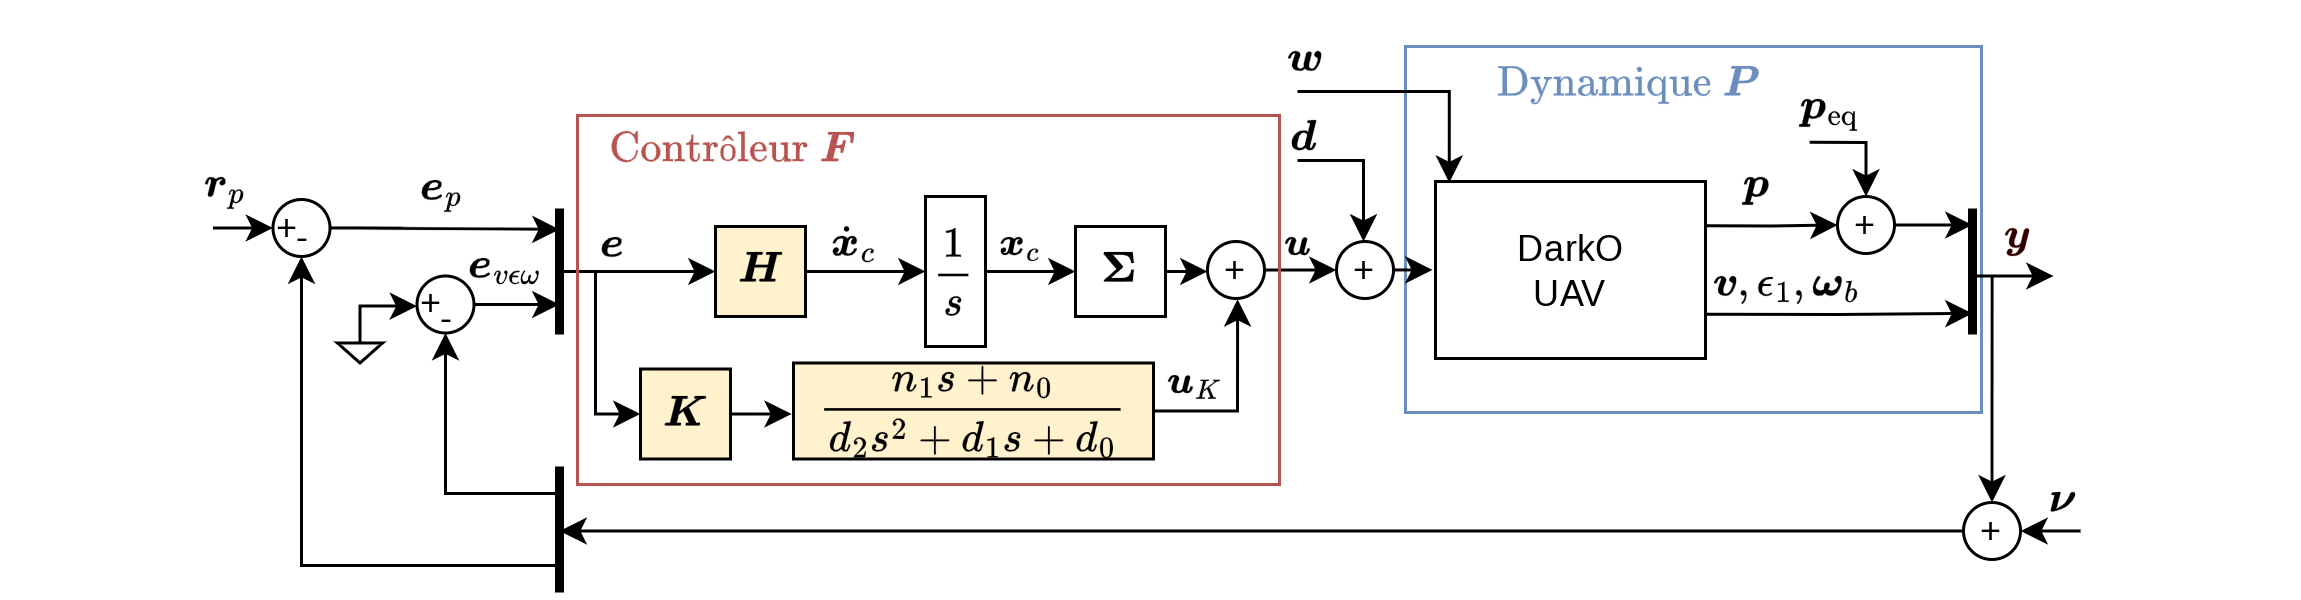
\includegraphics[width=1\columnwidth]{figures/commande_integrale.png}
    \caption{Schéma de commande intégralle avec la perturbation de vent $\boldsymbol{w}$, la perturbation du système à l'entrée $\boldsymbol{d}$ et à la sortie $\nu$.}
    \label{fig:commande_int6DOF}
\end{figure}

Comme le montre la figure~\ref{fig:commande_int6DOF}, les équations de la dynamique du contrôleur sont basées sur l'erreur $\boldsymbol{e}$ suivante :

\begin{subequations}
    \label{eq:contoller}
    \begin{align}
        \boldsymbol{e} = \smallmat{
        \boldsymbol{e}_{p}^\top & \boldsymbol{e}_{v\epsilon\omega}^\top}^\top, \quad \dot{\boldsymbol{x}}_{c} = \boldsymbol{H} \boldsymbol{e}, \quad    \boldsymbol{u} = \boldsymbol{\Sigma} \boldsymbol{x}_{c} + \boldsymbol{u}_{K},
        \\
        \boldsymbol{\Sigma} := \begin{bmatrix} \! 1 \!&\! 1\! & \!0\! &\! 0\!\\ \!0\! & \!0\! & \!1 \!& \!1\!\end{bmatrix}^\top, \quad
        \boldsymbol{u}_{K} = \frac{n_1 s+n_0}{d_2 s^{2}+d_1 s + d_0}\boldsymbol{K} \boldsymbol{e} ,
    \end{align}
\end{subequations}
où $\boldsymbol{x}_{c} \in \mathbb{R}^{2}$ est l'état intégral, $\boldsymbol{\Sigma}$ est une matrice d'allocation des entrées qui permet d'affecter la première composante de l'état de l'intégrateur à l'action des hélices et la deuxième composante à l'action des élevons. Les scalaires $n_1$, $n_0$,  $d_2$,  $d_1$,  $d_0$ sont respectivement les coefficients du numérateur et du dénominateur d'un filtre utilisé pour éviter une transmission directe entrée-sortie qui amplifierait le bruit de mesure à haute fréquence. Ce filtre induit un contrôleur strictement propre, pour une robustesse accrue aux incertitudes additives. Nous définissons le contrôleur $\boldsymbol{F}$ ayant pour dimensions 4\texttimes10 avec la matrice de transfert $\boldsymbol{F}(s) = T_{\boldsymbol{e} \rightarrow \boldsymbol{u}}(s)$ telle que décrite dans \eqref{eq:contoller} et l'interconnexion détaillé dans la figure~\ref{fig:commande_int6DOF}. Le système $\boldsymbol{P}$ de dimensions 10\texttimes4 représente la dynamique linéarisé de DarkO. La sortie du système $\boldsymbol{y} \in \real^{10\times1}$ est utilise comme entrée du controleur $\boldsymbol{F}$.

Compte tenu des symétries des actionneurs du drone, nous avons contraint la structure de la matrice $\boldsymbol{K}$ dans \eqref{eq:contoller}, associée à l'action proportionnelle du contrôleur, afin d'utiliser les actionneurs selon leur action physique. Ainsi, $\boldsymbol{K}$ prend la forme : 
\begin{align}
\label{eq:k_struct}
    \!\!\!\boldsymbol{K}_{\text{struct}} \!=\!  \smallmat{
             k_{1}& \shortminus k_{2}& k_{3}&  k_{4}& \shortminus k_{5}&  k_{6}& \shortminus k_{7}&  k_{8}&  k_{9}& \shortminus k_{10}\\
             k_{1}&  k_{2}& k_{3}&  k_{4}&  k_{5}&  k_{6}&   k_{7}& \shortminus k_{8}& \shortminus k_{9}&  k_{10}\\
            \shortminus k_{11}& \shortminus k_{12}& k_{13}& \shortminus k_{14}& \shortminus k_{15}& \shortminus k_{16}&   k_{17}& \shortminus k_{18}&  k_{19}& \shortminus k_{20}\\
            \shortminus k_{11}&  k_{12}& k_{13}& \shortminus k_{14}&  k_{15}&  k_{16}&   \shortminus k_{17}&  k_{18}&  k_{19}&  k_{20} 
         }.
\end{align}

La structure précédente s'explique par le comportement physique du drone, une erreur de position sur l'axe $z_{[\text{i}]}$ du repère inertiel NED (voir Fig.~\ref{fig:darko2}) entraîne une utilisation symétrique des deux hélices qui génère une force le long de l'axe $x_{[\text{b}]}$ du drone. L'utilisation symétrique des deux moteurs se traduit par le même signe dans les coefficients $k_{3}$ et $k_{6}$ des colonnes 3 et 6 de $\boldsymbol{K}$, correspondant respectivement aux erreurs de position et de vitesse sur l'axe $z_{[\text{i}]}$. De même, une erreur de position ou de vitesse le long de l'axe latéral du drone $y_{[\text{b}]}$ sera compensée par une utilisation antisymétrique des moteurs, comme le montrent les coefficients $k_{2}$ et $k_{5}$ et leurs signes opposés dans les colonnes 2 et 5 de $\boldsymbol{K}$. Une erreur de vitesse angulaire autour de l'axe $x_{[\text{b}]}$ doit être compensée par une utilisation antisymétrique des élevons, comme le montre le coefficient $k_{18}$ de signe opposé dans la colonne 8 de $\boldsymbol{K}$. Des arguments parallèles expliquent les coefficients restants de la matrice $\boldsymbol{K}$ dans \eqref{eq:k_struct}. Toute ces explications ne sont valable que dans un voisinage de l'équilibre, où le drone se trouve etre à la verticale. On comprends aisaiement que dans d'autre configuration, ces contraintes d'actionnement ne sont plus valable. Un avantage de la structure de \eqref{eq:k_struct} est la réduction du nombre de variables à optimiser, de 40 à 20 gains scalaires, cela traduisant pas une diminution du temps necessaire à l'optimisation.

La boucle fermée illustrée à la Fig.~\ref{fig:commande_int6DOF}, est un retour de sortie à 10 elements, comprenant les trois positions, les trois vitesses linéaires, l'un des trois angles d'attitude ($\epsilon_{1}$) et les trois vitesses angulaires. Cette structure peut être considérée comme un bouclage proportionnel-intégral MIMO. Les paramètres à régler dans le contrôleur $\boldsymbol{F}$ \eqref{eq:contoller} sont le gain proportionnel $\boldsymbol{K} \in \real^{4\times10}$ dans \eqref{eq:k_struct}, le gain intégral $\boldsymbol{H} \in \real^{2\times10}$ et les paramètres du filtre $n_1$, $n_0$, $d_2$, $d_1$, $d_0$, comme coloré en jaune sur la Fig.~\ref{fig:commande_int6DOF}. Une méthode de réglage appropriée doit garantir une rejection adéquate des perturbations et une robustesse satisfaisante aux dynamiques non modélisées. Ces deux objectifs conduisent à un compromis car le rejet des perturbations nécessite un réglage agressif tandis que les propriétés de robustesse sont assurées par une stratégie d'atténuation des hautes fréquences. Nous examinons ensuite deux méthodes de réglage basées sur l'optimisation. 
\todo{citer le paragphe précédent}
La première est issue des idées proposées dans \cite{SANSOUACA}, qui ne nécessitaient pas la dynamique linéarisée des Théorèmes~\ref{thm:eqs} et~\ref{th:lin}, et est résumée dans la section~\ref{sec:zerowind}. Il s'agit d'une synthèse multi-objectifs avec des contraintes $H_{\infty}$ basée sur le modèle de vent nul discuté dans la section~\ref{sec:eq_nowind} et~\ref{sec:nowind_lin} et dérivé dans \cite{SANSOUACA}.


Nous montrerons que cette première méthode ne permet pas de stabiliser le drone dans certaines plages de vent, en raison de la méconnaissance de la dynamique caractérisée par les Théorèmes~\ref{thm:eqs} et~\ref{th:lin}. La deuxième méthode de réglage, présentée à la section \ref{sec:h_inf6DOF_multi}, est une synthèse itérative multi-objectifs avec des contraintes $H_{\infty}$, basée sur un ensemble de modèles associés à différentes conditions de vent et dérivés des Théorèmes~\ref{thm:eqs} et~\ref{th:lin}, par le biais des Algorithmes~\ref{alg:eq} et~\ref{alg:linea}.


Dans notre validation numérique, présentée dans les sections~\ref{sec:zerowind} et~\ref{sec:h_inf6DOF_multi} (voir en particulier les Fig.~\ref{fig:SimSytuneStruct_zero} et Fig.~\ref{fig:SimSytuneStruct_lpv}), un bruit de mesure est ajouté à la sortie pour produire des résultats numériques semblable aux expérimentaux. Les écarts types des niveaux de bruit adoptés sont indiqués dans le tableau~\ref{tab:noise}.
\begin{table}[ht]
    \centering
    \begin{tabular}{|c|c|c|} 
        \hline
        Measurement & Value & Units\\
        \hline
        $\boldsymbol{p}$ & \SI{2.5e-4}{} & \SI{}{\meter}  \\ 
        \hline
        $\tilde{\boldsymbol{v}}$  & \SI{1.2e-3}{} &  \SI{}{\meter\per\second}  \\ 
        \hline
        $\tilde{\boldsymbol{\epsilon}}$ & \SI{4.7e-4}{} &  \\
        \hline
        $\tilde{\boldsymbol{\omega}}_{\text{b}}$ & \SI{2.7e-3}{} &\SI{}{\radian\per\second}\\
        \hline
    \end{tabular}
    \caption{ Écart-type du bruit pour la modélisation des capteur en simulation.}
    \label{tab:noise}
\end{table}

En plus de présenter les résultats de la simulation du bouclage linéaire de la Fig. ~\ref{fig:commande_int6DOF} avec le modèle linéarisé \eqref{eq:lpv_linearisation}, dans les sections~\ref{sec:zerowind} et~\ref{sec:h_inf6DOF_multi}, nous simulons également la boucle fermée en remplaçant le modèle linéarisée $\boldsymbol{P}$ par le modèle non linéaire \eqref{eq:dyna_orig}, comprennant la dynamique réélle du drone.

Lorsque l'on remplace le modèle linéarisée par la dynamique non linéaire \eqref{eq:dyna_orig}, dont l'état est $\boldsymbol{x} = (\boldsymbol{p}, \boldsymbol{v}, \boldsymbol{q},\boldsymbol{\omega}_{\text{b}}) \in \real^{13} $,
nous remplaçons la sortie linéaire $\boldsymbol{y}$ par la version non linéaire suivante $\boldsymbol{x} = (\boldsymbol{p}, \boldsymbol{v},\boldsymbol{q},\boldsymbol{\omega}_{\text{b}}) \in \real^{13} $. 
De plus, nous remplaçons la sortie lineaire $\boldsymbol{y}$ avec la version non linéaire suivante:
\begin{align}
\label{eq:output}
    \boldsymbol{y}_{\text{NL}} \!=\! \smallmat{\boldsymbol{p}\\
     \boldsymbol{v}\\
     \epsilon_{1}\\
     \boldsymbol{\omega}_{\text{b}}} \!=\! \left[ \begin{smallmatrix} \mathbb{I}_{6} & \mathbb{0}_{6\times 1} & \mathbb{0}_{6\times 1} & \mathbb{0}_{6\times 2} & \mathbb{0}_{3}\\
     \mathbb{0}_{1\times 3} & 0 & 1 & \mathbb{0}_{1\times 2} & \mathbb{0}_{1 \times 3} \\
         \mathbb{0}_{3} & \mathbb{0}_{3\times 1} & \mathbb{0}_{3\times 1} & \mathbb{0}_{3\times 2} &   \mathbb{I}_{3}
         \end{smallmatrix} \right]
         \smallmat{\boldsymbol{R}^\top_{\psi}\boldsymbol{p} \\ \boldsymbol{R}^\top_{\psi}\boldsymbol{v} \\
\boldsymbol{q}_{\mathrm{eq}\psi}^{-1} \otimes \boldsymbol{q} \\
         \boldsymbol{\omega}_{\text{b}}  }.
\end{align}


Dans les sections suivantes, nous notons la marge de module d'une matrice de transfert $s \mapsto T_{v \rightarrow z}$ as $\Delta_m(T_{v \rightarrow z}) = \min\limits_{\omega\in R} \sigma_{\min}(T_{v \rightarrow z}(j\omega))$.



\subsection{Controleur optimisé sous contrainte $H_{\infty}$, cas sans vent}
\label{sec:zerowind}

Pour régler le controleur dans le cas sans vent, nous utilisons le modèle linéaire du système décrit dans la section~\ref{sec:nowind_lin}, $\boldsymbol{P}(s) = T_{\boldsymbol{u} \rightarrow \boldsymbol{y}}(s)$, obtenue à partir des équations \eqref{eq:linearized} et \eqref{eq:output_lin} tel que :

\begin{align*}
    \boldsymbol{P}(s) = \boldsymbol{C} (s \mathbb{I}_{12} - \boldsymbol{A}_{0})^{-1} \boldsymbol{G}_{0}.
\end{align*} 

En lien avec la figure~\ref{fig:commande_int6DOF}, nous introduisons des matrices de transfert qui correspondent aux objectifs de robustesse : la fonction de sensibilité en sortie définie par $T_{\nu \rightarrow e}=(\mathbb{I}_{10}+\boldsymbol{P}\boldsymbol{F})^{-1}$ de dimension 10\texttimes10, telle que $\lVert T_{\nu \rightarrow e} \rVert _{\infty}=\Delta_m(T_{\nu \rightarrow e})^{-1} $ et la fonction de sensibilité en entrée $T_{d \rightarrow u}=(\mathbb{I}_{4}+\boldsymbol{F}\boldsymbol{P})^{-1}$ de dimension 4\texttimes4, définie par $\lVert T_{d \rightarrow u} \rVert _{\infty}=\Delta_m(T_{d \rightarrow u})^{-1}$.
Par conséquent, la minimisation de la norme $H_{\infty}$ de $T_{\nu \rightarrow e}$ ou de $T_{d \rightarrow u}$ correspond à l'augmentation des marges de module en entrée et en sortie. Étant donné que le système $\boldsymbol{P}$ est MIMO, nous accordons de l'importance aux fonctions de sensibilité en entrée et en sortie qui ne coïncident pas, car $\boldsymbol{P}$ et $\boldsymbol{F}$ ne commute pas.

Nous definnisons aussi la mtrice de tranfert $T_{\nu \rightarrow u}$ de dimensions 4\texttimes10 lié à l'impact du bruit de mesure $\nu$ sur la commande $\boldsymbol{u}$, e $T_{d \rightarrow y}$ de dimensions 10\texttimes4 représentant l'impact de la perturbation en entrée $\boldsymbol{d}$ sur la sortie du systeme $\boldsymbol{y}$. 

Nous résolvons le même problème que dans notre travail précédent \ref{eq:pb_optim} en utilisant le logiciel {\tt Systune} \cite{1576856}, mais nous utilisons le diagramme de contrôle présenté dans la section~\ref{sec:ctl_sche} qui comprend un filtre sur l'action proportionnelle et un nombre différent de sorties. Nous incluons également dans le système $\boldsymbol{P}$ la dynamique des actionneurs linéaires discutée dans la section~\ref{sec:saturation}.
\begin{figure}[b!]
    \centering
    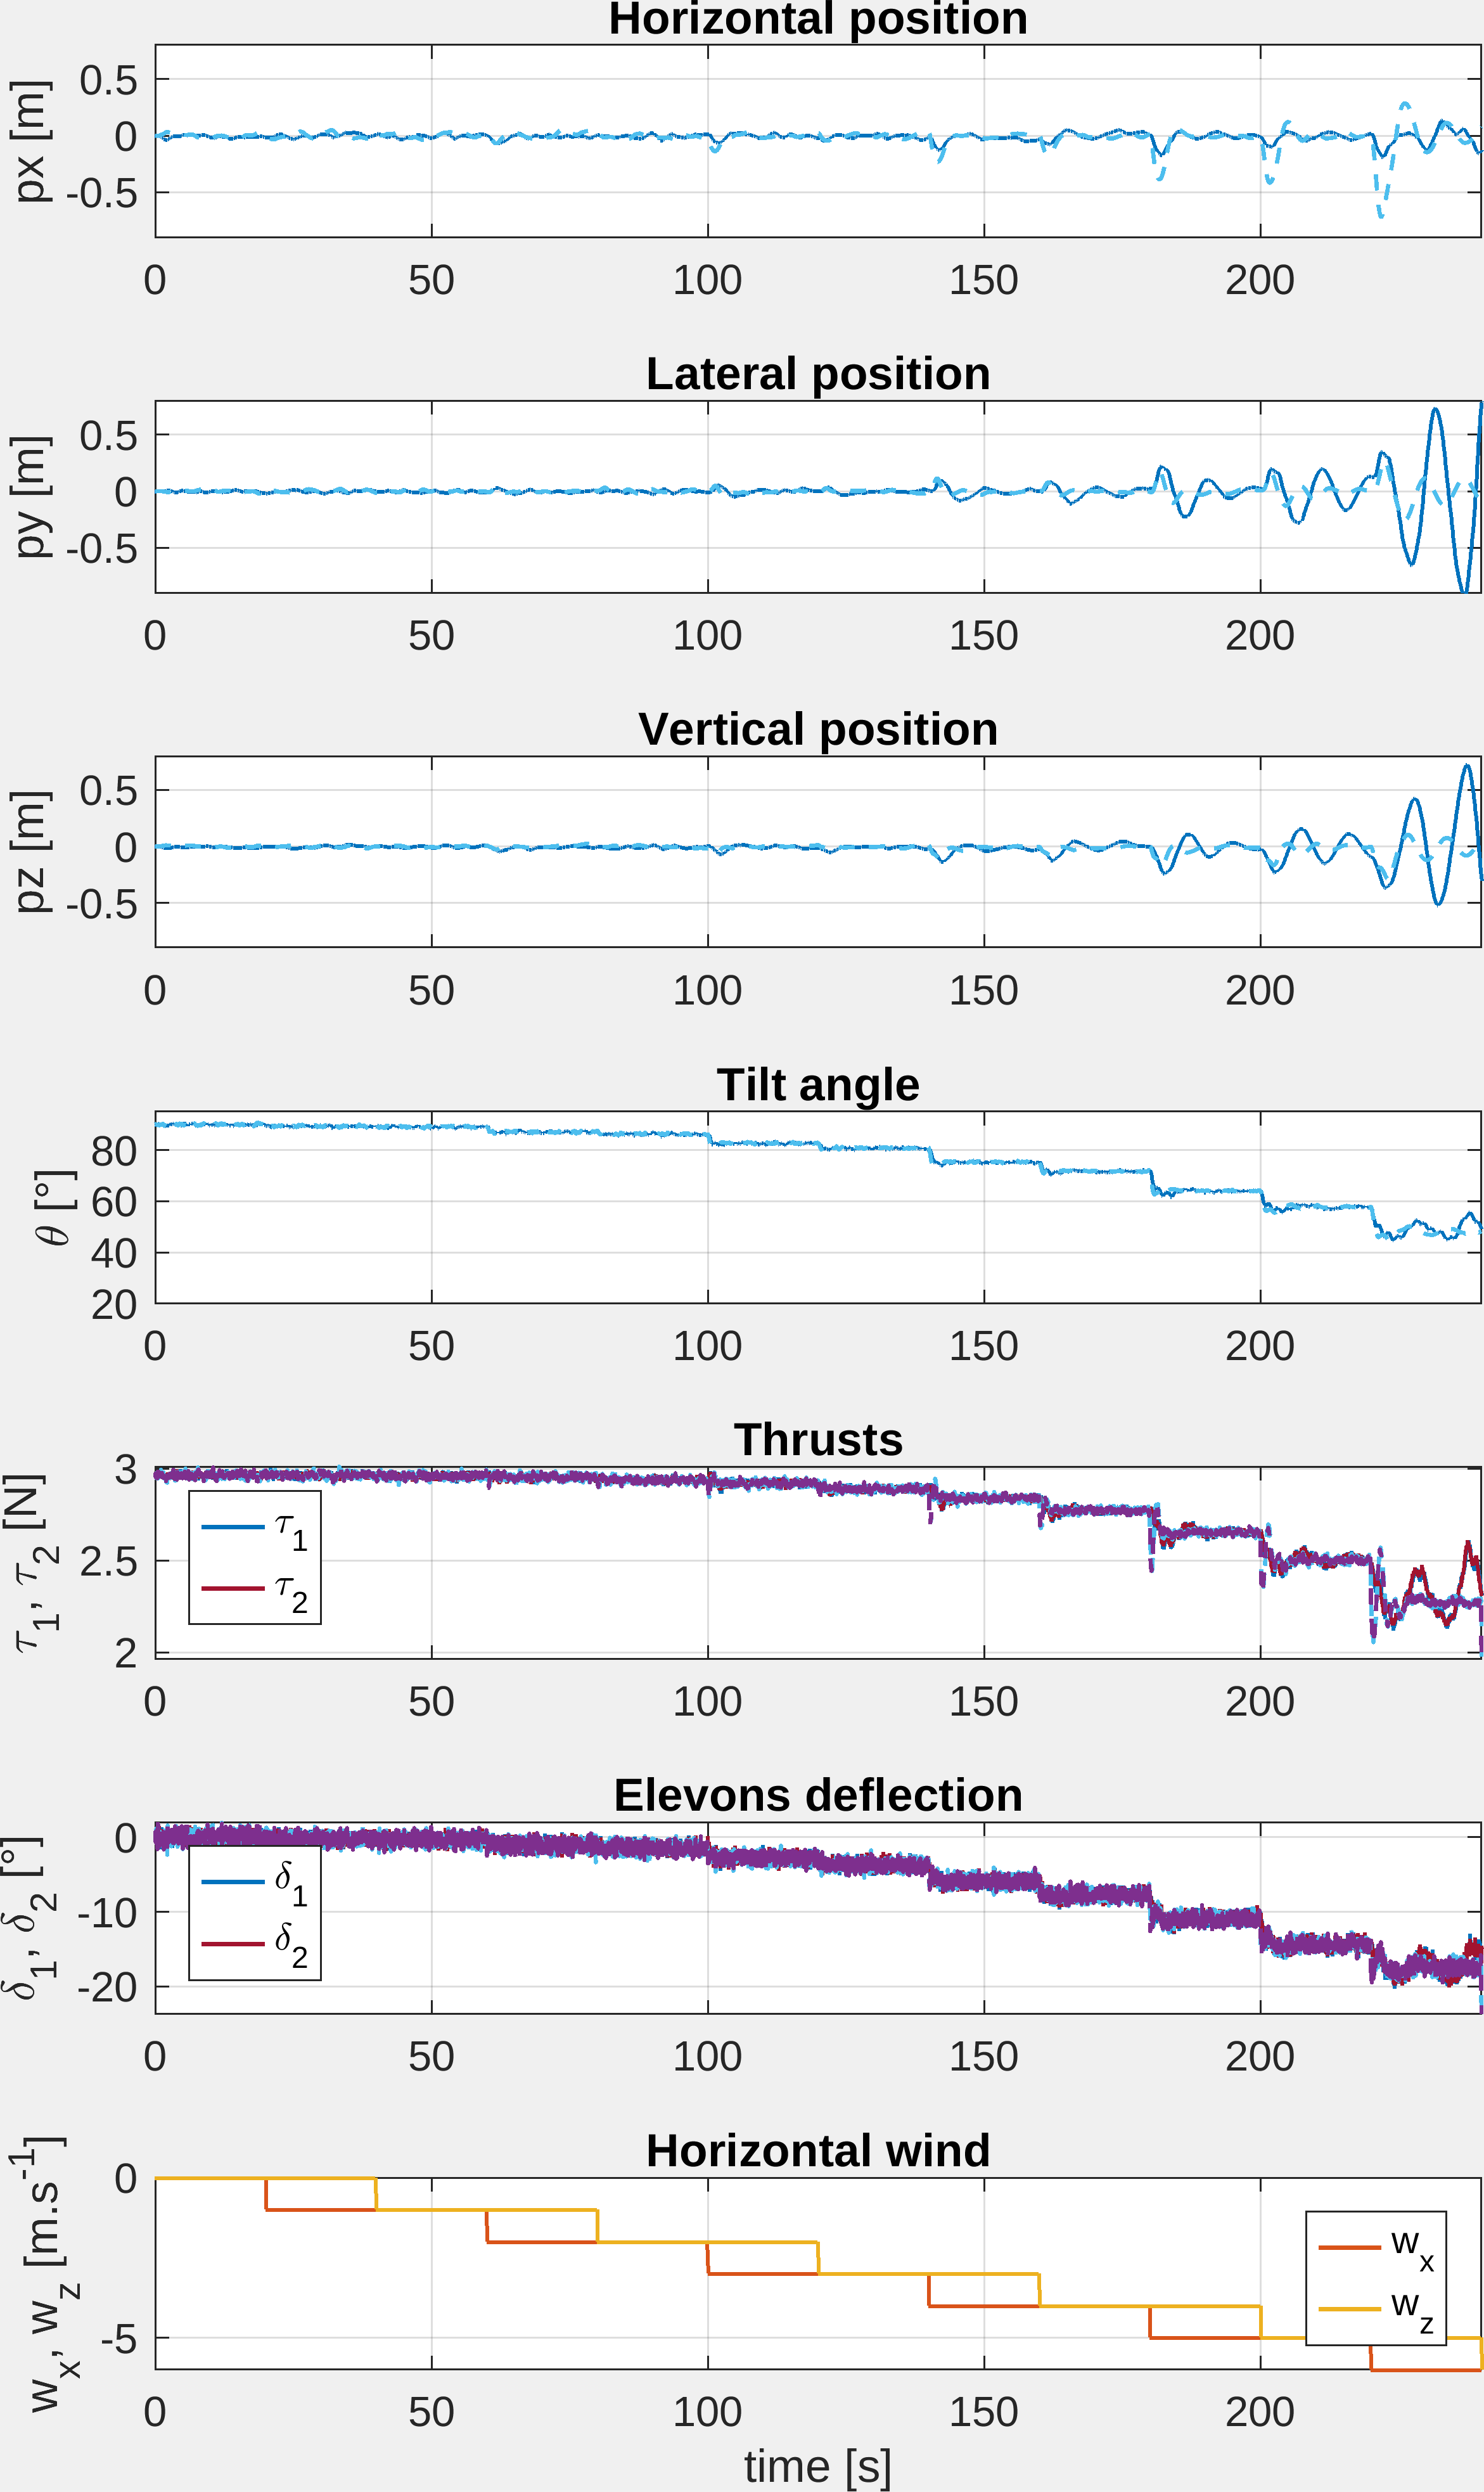
\includegraphics[trim=0cm 0cm 0cm 0cm,clip,width=0.9\columnwidth]{figures/sim_systune_zero_wind.png}
    \caption{Simulation of the non-linear model \eqref{eq:dyna_orig} (solid line) and the linearized model \eqref{eq:lpv_linearisation} (dashed line) with increasing constant wind steps with the controller tuned using the zero-wind optimization of Section~\ref{sec:zerowind}.}
    \label{fig:SimSytuneStruct_zero}
\end{figure}

Une augmentation successive de l'intensité horizontale et verticale du vent (allant de zéro à \SI{-6}{\meter\per\second}) sont appliquées, comme le montre le tracé inférieur de la Fig.~\ref{fig:SimSytuneStruct_zero}. Les couples de vents sélectionnées $(w_{x}, w_{z})$ sont représentées par des points rouges sur les surfaces de la figure~\ref{fig:saturation}, où l'on peut voir que l'équilibre $(\boldsymbol{u}_{\text{eq}}, \boldsymbol{x}_{\text{eq}})$ est atteint sans que les actionneurs ne soient saturés. Nous ne nous intéressons qu'à la partie négative de la vitesse verticale du vent car elle est la plus limitante. En effet, le drone est soulevé par le vent vertical ascendant (dont le signe est négatif dans le cadre de la NED), il a donc besoin de moins de traction sur les hélices pour compenser la gravité. Les moteurs génèrent moins de flux d'air sur les élevons, ce qui réduit leur efficacité, conduit à la saturation et déstabilise le drone.
L'objectif du système de contrôle est de maintenir le drone en position de vol stationnaire (définie comme $\boldsymbol{r}_{p} = [0,0,0]^\top$), malgré l'augmentation du vent horizontal et vertical $w_{x}$ et $w_{z}$. 


La figure~\ref{fig:SimSytuneStruct_zero} présente à la fois des simulations linéaires avec la dynamique linéarisée \eqref{eq:lpv_linearisation} (en traits pointillés) et des simulations non linéaires avec le modèle non-linéaire \eqref{eq:dyna_orig} (en traits pleins). Les simulations linéaires et non linéaires montrent systématiquement que le contrôleur fonctionne bien à faible vitesse de vent (effectivement, le réglage est effectué sur la base du modèle de vent nul). Cependant, lorsque la vitesse du vent $w_{x}$ et $w_{z}$ dépasse \SI{-5}{\meter\per\second}, la position de vol stationnaire devient instable et le drone oscille et diverge. Les angles d'inclinaison $\theta$ sont utilisés pour représenter l'attitude afin de donner un meilleur aperçu du comportement du véhicule, mais la simulation de la dynamique non linéaire \eqref{eq:dyna_orig} est effectuée avec un quaternion unitaire. L'instabilité observée dans les résultats de la simulation de la figure~\ref{fig:SimSytuneStruct_zero} confirme les instabilités expérimentales rapportées dans la section \ref{sec:exp3DOF} où nous avons utilisé cette même méthode de réglage, et confirme l'importance des Théorèmes~\ref{thm:eqs} et~\ref{th:lin} dans la Section~\ref{sec:model}, pour un réglage approprié des gains du contrôleur, ce qui est effectué dans la section suivante.


\subsection{\texorpdfstring{Controleur optimisé sous contrainte $H_{\infty}$}{H {infty}}, cas multimodèle}
\label{sec:h_inf6DOF_multi}

The simulation results obtained with the zero-wind tuning method (see Fig.~\ref{fig:SimSytuneStruct_zero}) together with the experimental instabilities observed in \cite{SANSOUACA} confirm the need for a controller gain tuning procedure exploiting the parametrized non-zero wind linearizations of Theorems~\ref{thm:eqs} and~\ref{th:lin}. Focusing again on the control scheme of Fig.~\ref{fig:commande_int6DOF}, we now explicitly consider the (linearized) wind effect on the plant, and we consider the linearized plant dynamics \eqref{eq:lpv_linearisation} with output \eqref{eq:output_lin} and with the selections in Algorithm~\ref{alg:linea} as
\begin{align*}
\label{eq:Pw_synthesis}
\numberthis
    \boldsymbol{P}_w(s) &= \begin{bmatrix}
        \boldsymbol{P}_{u}(s;w) &  \boldsymbol{P}_{w}(s;w)
    \end{bmatrix}\\&:= \boldsymbol{C} (s \mathbb{I}_{12} - \boldsymbol{A}_{w})^{-1} \begin{bmatrix}\boldsymbol{G}_{w} &   \boldsymbol{E}_{w}\end{bmatrix},
\end{align*}
whose input is the concatenation of the control input $\boldsymbol{u}$ and the wind disturbance input $\boldsymbol{w}$. As the model depends on the wind speed $\boldsymbol{w}$, we introduce a new transfer matrix $T_{w \rightarrow y}$ having dimensions 10\texttimes3, which corresponds to the transfer matrix between the wind input $\boldsymbol{w}$ and the plant output $\boldsymbol{y}$, quantifying the effect of the wind disturbance on the UAV feedback loop. 
%
With the set of transfers matrices defined in Sec.~\ref{sec:zerowind} and the new transfer matrix $T_{w \rightarrow y}$, we use the algorithmic 
approach in \cite{1576856,ApkarianMulti}, named ``{\tt systune}'', which uses non-smooth optimization techniques to deal with non-convex tuning problems, 
such as our structured control architecture where we optimize the gain matrices $\boldsymbol{K}$, $\boldsymbol{H}$ and the filter parameters $n_1$, $n_0$,  $d_2$,  $d_1$,  $d_0$ (in yellow on the figure~\ref{fig:commande_int6DOF}).
As reported in  \cite[eq. (2)]{ApkarianMulti}, 
we solve a multi-objective optimization problem,
by exploiting the Matlab implementation well explained in \cite[\S 3]{ApkarianMulti}.
%
In particular, based on a set ${\mathcal W}$ comprising a finite collection of pairs $(w_x, w_z)$, with 
$w_{x} \in [0,~8]~\SI{}{\meter\per\second}$ and $ w_{z} \in [\shortminus 4,~4]~\SI{}{\meter\per\second}$,
we consider the ensuing set of linearized plants \eqref{eq:Pw_synthesis}
and solve the following convex optimization, where
scalars $W_{1}$, $W_{2}$, $W_{3}$, $W_{4}$ and $W_{5}$ are weighting factors to be tuned to obtain a satisfactory trade-off between robustness (associated with $W_2$, $W_3$ and $W_4$) %(roll-off strategy and minimising the module margin) 
and performance (associated with $W_1$ and $W_5$) %(bring $\boldsymbol{e}$ to zero despite the low frequency disturbance $\boldsymbol{w}$). 
\begin{align*} \label{eq:pb_optim_lpv}
\numberthis
\gamma^\star &= \min_{\boldsymbol{F}} \max_{w \in {\mathcal W}} 
\begin{vmatrix}
    \| W_{1} T_{\nu \rightarrow e}(\boldsymbol{P}_w,\boldsymbol{F})\|_{\infty} \\
    \|W_{2} T_{d \rightarrow u}(\boldsymbol{P}_w,\boldsymbol{F})\|_{\infty}\\
    \|W_{3} T_{\nu \rightarrow u}(\boldsymbol{P}_w,\boldsymbol{F})\|_{\infty}\\
    \|W_{4} T_{d \rightarrow y}(\boldsymbol{P}_w,\boldsymbol{F})\|_{\infty}\\
    \|W_{5} T_{w \rightarrow y}(\boldsymbol{P}_w,\boldsymbol{F})\|_{\infty}
    \end{vmatrix}_{\infty}, \text{ subject to} \\ 
    &\qquad \boldsymbol{F}
    \text{ stabilizes internally } {\mathcal F}_\ell (\boldsymbol{P}_w,\boldsymbol{F}), \forall w \in {\mathcal W},
\end{align*}
where ${\mathcal F}_\ell(\boldsymbol{P}_w,\boldsymbol{F})$ denotes the linear feedback interconnection of Fig.~\ref{fig:commande_int6DOF}
for a specific value of $w$ (this is consistent with the classical robust control notation \cite{1576856,ApkarianMulti}).
%
Notice that, with reference to \cite[eq. (2)]{ApkarianMulti}, we only specify soft constraints and we do not specify any hard constraint.

% it is possible to construct the following minimization problem:
% \begin{align*} \label{eq:pb_optim_lpv}
% &\min_{\boldsymbol{F}}\quad \begin{Vmatrix}
%     W_{1} T_{\nu \rightarrow e}(\boldsymbol{P}_w,\boldsymbol{F})\\
%     W_{2} T_{d \rightarrow u}(\boldsymbol{P}_w,\boldsymbol{F})\\
%     W_{3} T_{\nu \rightarrow u}(\boldsymbol{P}_w,\boldsymbol{F})\\
%     W_{4} T_{d \rightarrow y}(\boldsymbol{P}_w,\boldsymbol{F})\\
%     W_{5} T_{w \rightarrow y}(\boldsymbol{P}_w,\boldsymbol{F})
%     \end{Vmatrix}_{\infty}, \text{ subject to} \\ & \boldsymbol{F} \in \mathbb{R}^{10 \times 4} \text{ stabilizes } \boldsymbol{P}_w \text{ internally,} \numberthis
% \end{align*}
% where $\boldsymbol{P}_w$ parametrizes a finite set of linear models evaluated at the points $w_{x} \in \{0,~2,~4,~6,~8\}~\SI{}{\meter\per\second}$ and $ w_{z} \in \{\shortminus 4,~\shortminus2,~0,~2,~4\}~\SI{}{\meter\per\second}$. We determined the linearisation of the model for each wind condition using equation~\eqref{eq:lpv_linearisation} to create $\boldsymbol{P}_w$, connected in feedback with controller $\boldsymbol{F}$ as in Fig.~\ref{fig:commande_int6DOF} and \eqref{eq:output_lin} \eqref{eq:contoller}. The 

\begin{algorithm}
  \caption{Iterative multimodel controller gain tuning.}
  \label{alg:iterativeOptimisation}
  \hspace*{.1cm} \textbf{Input}: $\boldsymbol{A}_{w}$, $\boldsymbol{G}_{w}$, $\boldsymbol{E}_{w}$  the output matrices of Algorithm~\ref{alg:linea} and the positive weighting scalars $W_1$--$W_5$\\
  \hspace*{.1cm} \textbf{Output}: $\boldsymbol{K}$, $\boldsymbol{H}$ and the filter gains
  \begin{algorithmic}[1]
   
    \State (Initialization) Initialize ${\mathcal W}$ as a grid comprising all the pairs $ w_{x} \in \{0,~-4,~-8\}$ and $ w_{z} \in \{\shortminus 4,~0,~4\}$
    \State \label{step:synthesis} (Synthesis) Solve the optimization \eqref{eq:pb_optim_lpv} with the software {\tt systune}

    \State \label{step:analysis} (Analysis) Define a validation grid ${\mathcal W}_{\text{v}}$ by discretizing the interval $(w_x,w_y) \in [0,8]\times[-4,4]$ with a discretization step of $1$ and 
    using the controller $\boldsymbol{F}$ obtained from the previous step, compute, for each $w_{\text{v}}\in {\mathcal W}_{\text{v}}$,
    \begin{align}
    \label{eq:validation_step}
    \gamma_{\text{v}} = \begin{vmatrix}
    \| W_{1} T_{\nu \rightarrow e}(\boldsymbol{P}_{w_{\text{v}}},\boldsymbol{F})\|_{\infty} \\
    \|W_{2} T_{d \rightarrow u}(\boldsymbol{P}_{w_{\text{v}}},\boldsymbol{F})\|_{\infty}\\
    \|W_{3} T_{\nu \rightarrow u}(\boldsymbol{P}_{w_{\text{v}}},\boldsymbol{F})\|_{\infty}\\
    \|W_{4} T_{d \rightarrow y}(\boldsymbol{P}_{w_{\text{v}}},\boldsymbol{F})\|_{\infty}\\
    \|W_{5} T_{w \rightarrow y}(\boldsymbol{P}_{w_{\text{v}}},\boldsymbol{F})\|_{\infty}
    \end{vmatrix}_{\infty} ,
    \end{align}
    and augment ${\mathcal W}$ with the corresponding point if $\gamma_{\text{v}} > 1$ or $\gamma_{\text{v}}$ is undefined (namely if $\boldsymbol{F}$ is not internally stabilizing).

    \State (Termination) If ${\mathcal W}$ has not been augmented at the previous step, then move to step~\ref{step:final}, otherwise move to step~\ref{step:synthesis}.
    
    \State \label{step:final} 
    \textbf{Return:} $\boldsymbol{K}$, $\boldsymbol{H}$ and filter parameters $n_1$, $n_0$,  $d_2$,  $d_1$,  $d_0$
    
    % \textbf{if} a transfer does not satisfy constraints \textbf{then}
    %      \NoNumber{\quad Add point to the optimization grid} 
    %      \NoNumber{\quad New iteration of Step 2} \\
    % \textbf{else} 
    %     \NoNumber{\quad \textbf{Return:} $\boldsymbol{K}$, $\boldsymbol{H}$ and filter parameters $n_1$, $n_0$,  $d_2$,  $d_1$,  $d_0$}
  \end{algorithmic}
\end{algorithm}

The optimization problem \eqref{eq:pb_optim_lpv} becomes increasingly cumbersome, from a computational viewpoint, as we increase the cardinality of the set of wind conditions considered in ${\mathcal W}$. In fact, a brute force approach including a fine grid of points in ${\mathcal W}$ leads to a computationally intractable optimization. Instead, we follow here the
iterative procedure overviewed in Algorithm~\ref{alg:iterativeOptimisation}, 
where ${\mathcal W}$ is initially selected as a sparse grid comprising $3 \times 3 = 9$ points (step 1) and then 
a synthesis step (step 2) is repeatedly followed by a (computationally simple) analysis step (step 3) where controller $\boldsymbol{F}$ is fixed.
Step 3 identifies the violating points by using a finer validation grid ${\mathcal W}_{\text{v}}$ and adds them to 
the optimization set ${\mathcal W}$. The algorithm terminates after some iterations, when no points of the validation grid violate the constraints.

\begin{table}
    \centering
    \begin{tabular}{|l|c|c|c|c|c|} 
    \hline
    Weighting scalars & $W_1$ & $W_2$ & $W_3$ & $W_4$ & $W_5$ \\ \hline
    Values &18 & 16 & 11 & 26 & 5 \\ \hline
    \end{tabular}
    \label{tab:W1-W5}
    \caption{Values of the positive weighting scalars $W_1$--$W_5$ used in the execution of Algorithm~\ref{alg:iterativeOptimisation}.}
\end{table}

Executing Algorithm~\ref{alg:iterativeOptimisation} for the DarkO models of Theorems~\ref{thm:eqs} and~\ref{th:lin} with the selection
of the positive weighting scalars $W_1$--$W_5$ reported in Table~\ref{tab:W1-W5}, returned the following selection after 2 iterations:
\begin{align*}
 \left[\!\! \begin{array}{c|c} 
 \boldsymbol{K}^\top \!\!&  \boldsymbol{H}^\top \!\!
       \end{array} \right] \!&=\!
\left[\!\! \begin{array}{c|c} 
\begin{smallmatrix}
    -3.86&-3.86&0.79&0.79\\ 
1.43&-1.43&1.71&-1.71\\ 
4.06&4.06&-2.07&-2.07\\ 
-6.86&-6.86&-11.60&-11.60\\ 
-10.75&10.75&-1.89&1.89\\ 
27.20&27.20&-4.29&4.29\\ 
-12.32&12.32&-3.46&3.46\\  
-5.84&5.84&-2.29&2.29\\ 
-5.19&5.19&5.79&5.79\\ 
-6.52&6.52&0.08&-0.08\\ 
\end{smallmatrix}&
\begin{smallmatrix}
    0.02&0.48\\ 
    -0.47&-1.63\\ 
    -0.45&0.52\\ 
    -0.14&1.40\\ 
    3.35&5.69\\ 
    -1.84&3.79\\ 
    3.72&6.81\\ 
    1.58&3.13\\ 
    2.86&-1.54\\ 
    0.08&2.82\\ 
\end{smallmatrix}
\end{array} \right],\\
\left[\!\! \begin{array}{c|c} 
        n_1 &  n_0\\ \hline
        d_2 &  d_1\\\hline
        d_0 &  
       \end{array} \right] \!&=\!
       \left[\begin{array}{c|c} 
        \smallm{-429} & \smallm{-389}\\ \hline
        \smallm{1} &  \smallm{6475}\\ \hline
        \smallm{4905} &  
       \end{array}\right],
       \numberthis
       \label{eq:gain_selection}
\end{align*}

For the first iteration of Algorithm~\ref{alg:iterativeOptimisation}, after a candidate controller $\boldsymbol{F}$ has been evaluated at step~\ref{step:synthesis},
Fig.~\ref{fig:transferts_tcst} shows in blue the bode diagrams of the maximum singular values of $T_{\nu \rightarrow e}$, $T_{d \rightarrow u}$, 
$T_{\nu \rightarrow u}$, $T_{d \rightarrow y}$, and $T_{w \rightarrow y}$ (associated with the value of $\gamma_{\text{v}}$) 
reported in \eqref{eq:validation_step} at the analysis step~\ref{step:analysis}, to be compared to the inverse of the five weights $W_1$--$W_5$, represented by the green horizontal lines. The diagrams in red correspond to the points that violate the constraints and that are added to the set ${\mathcal W}$ for the next iteration. The few diagrams in magenta, instead, correspond to the 9 points considered in ${\mathcal W}$ for the first iteration of the synthesis step~\ref{step:synthesis}.
The red diagrams in Fig.~\ref{fig:transferts_tcst} clearly illustrate that the iterative algorithm manages to detect the critical values of wind speed $(w_x,w_z)$ to be added to the optimization set
 ${\mathcal W}$.


The singular values of the output and the input sensitivity function (respectively $T_{r \rightarrow e}$ and $T_{d \rightarrow u}$)  are shown in Fig.~\ref{fig:transferts_tcst} top line. The graph in the third line represents the singular value of the transfer between the wind disturbance $\boldsymbol{w}$ and the drone output $\boldsymbol{y}$. The singular value tangent to the constraint is that for the highest wind condition a.g.  $(w_x, w_z) = (-8,-4)~\SI{}{\meter\per\second}$.








\begin{figure}[ht!]
    \centering
    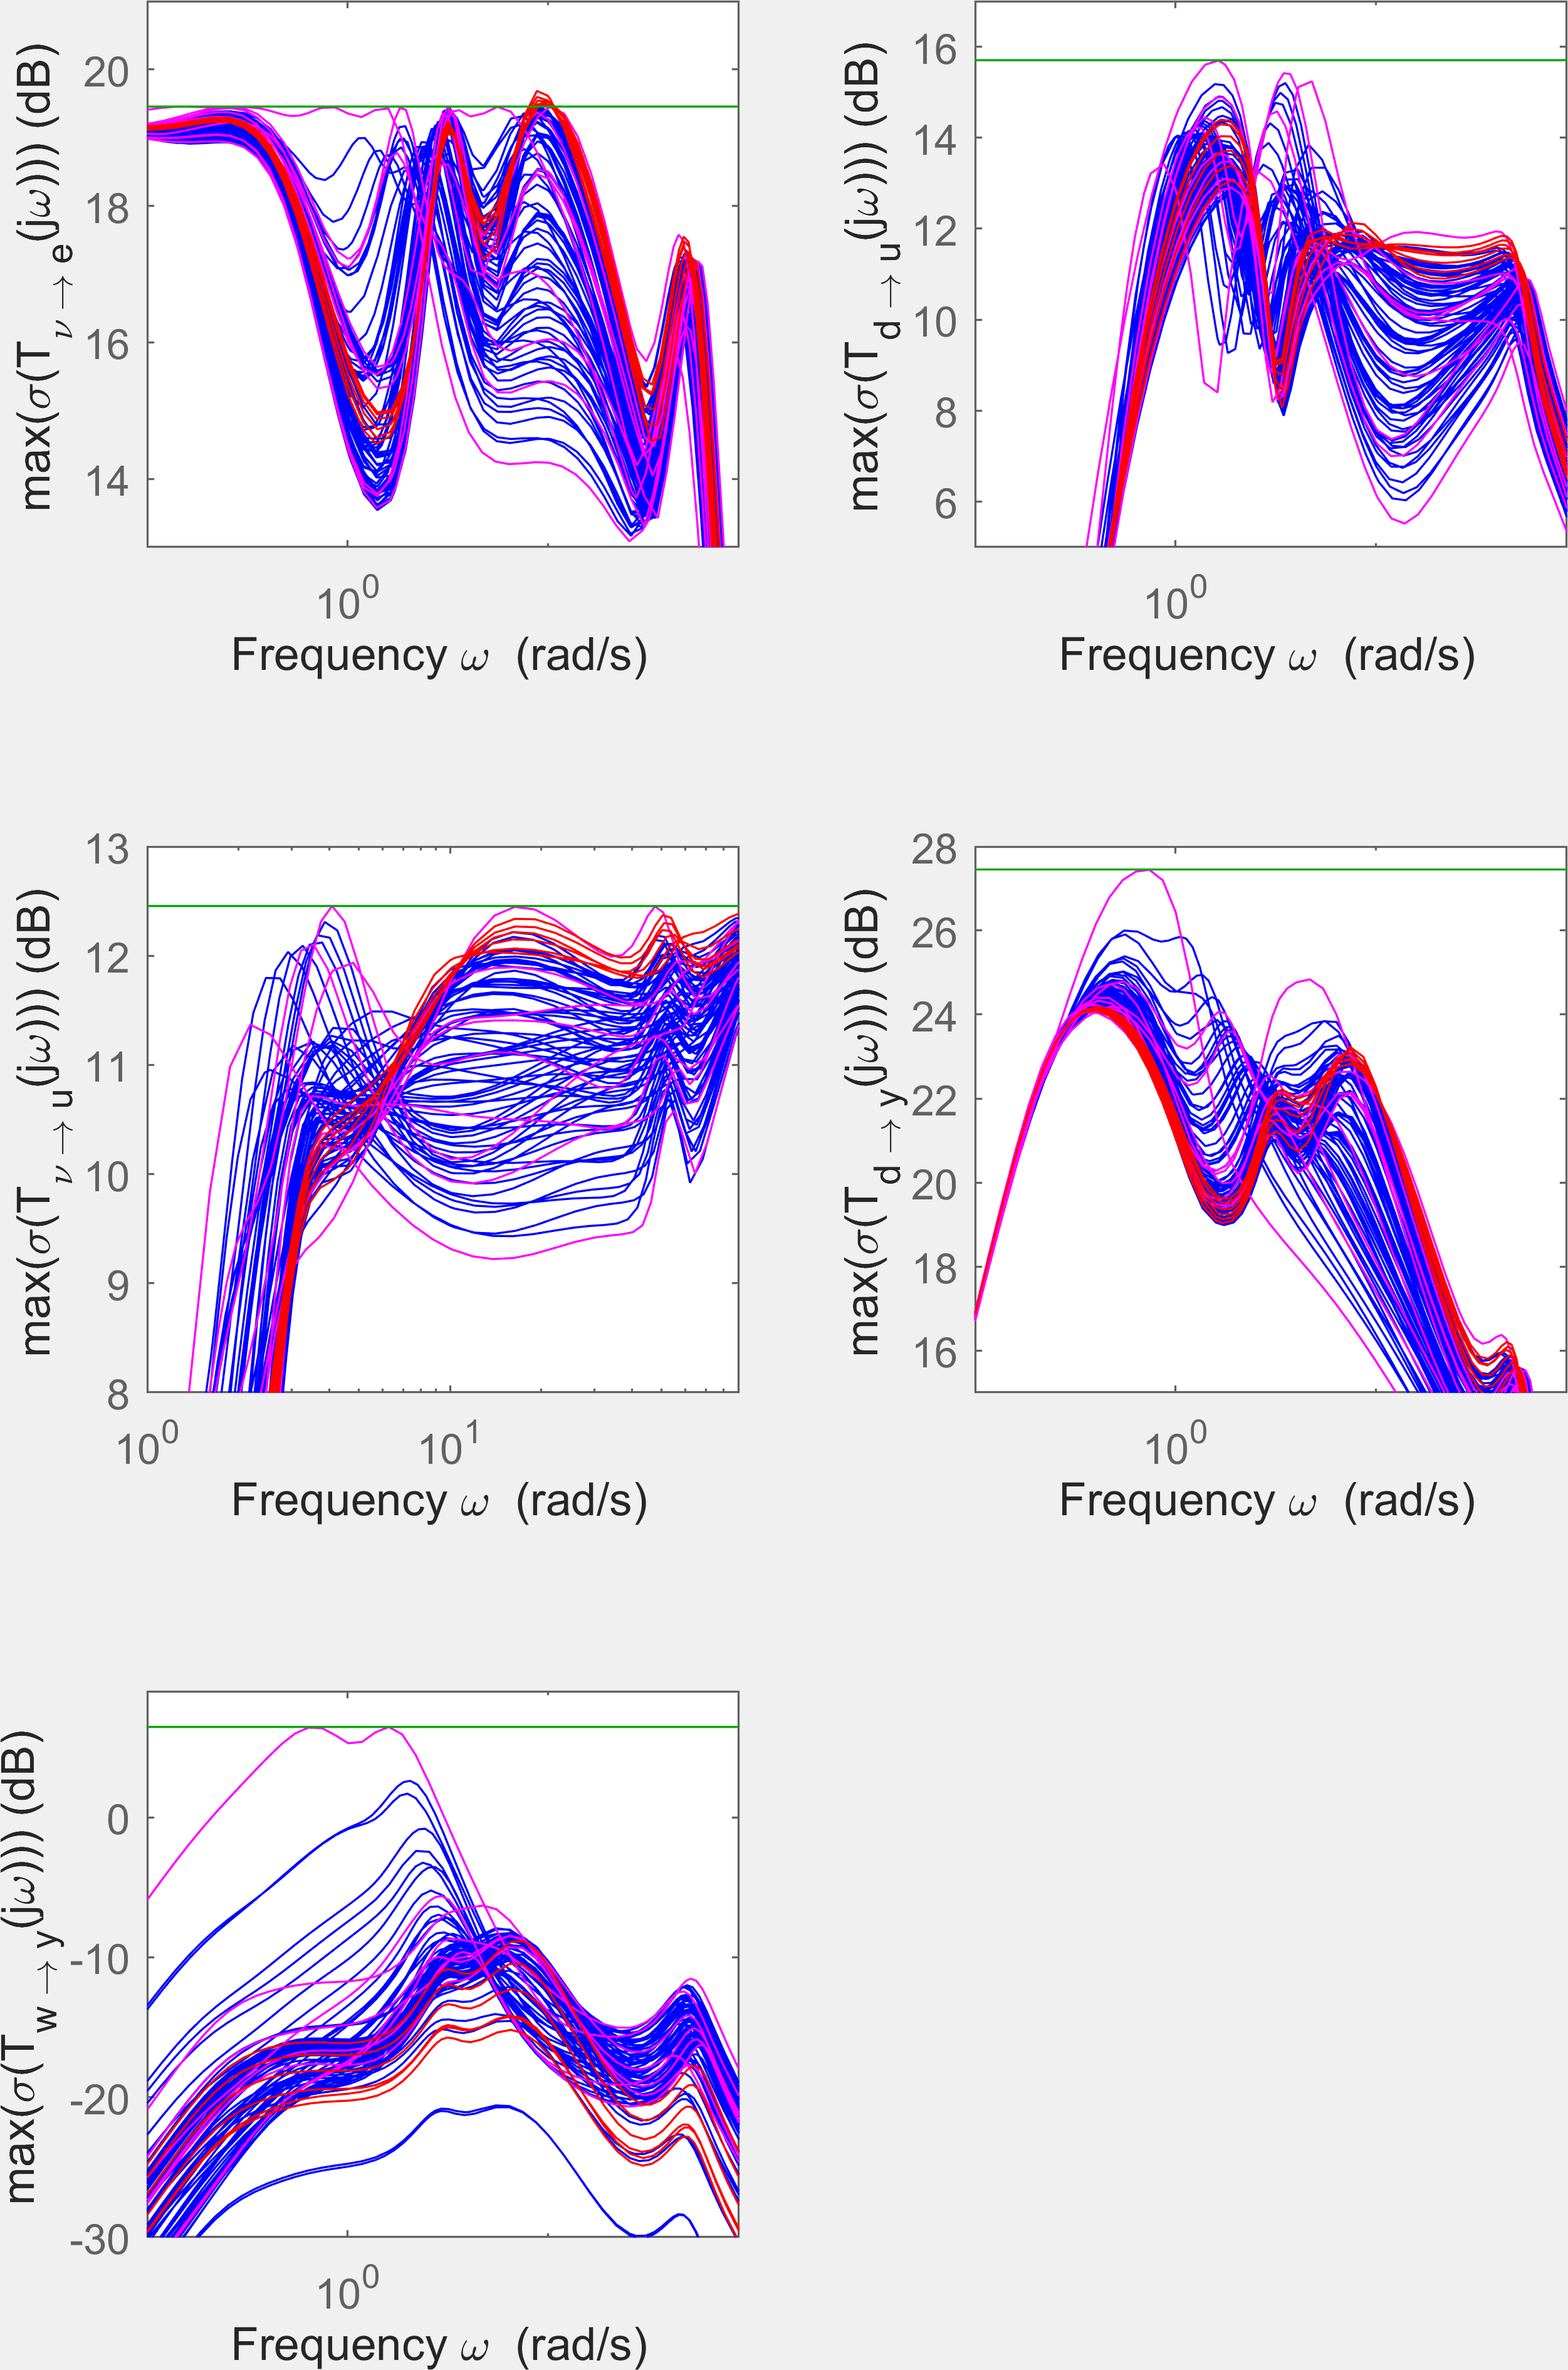
\includegraphics[trim=0cm 0cm 0cm 0cm,clip,width=0.9\columnwidth]{figures/transferts_tcst.png}
    \caption{Diagrams of the singular values of the transfer functions in \eqref{eq:validation_step} at the first iteration of Algorithm~\ref{alg:iterativeOptimisation}.}
    \label{fig:transferts_tcst}
\end{figure}


\begin{figure}[ht!]
    \centering
    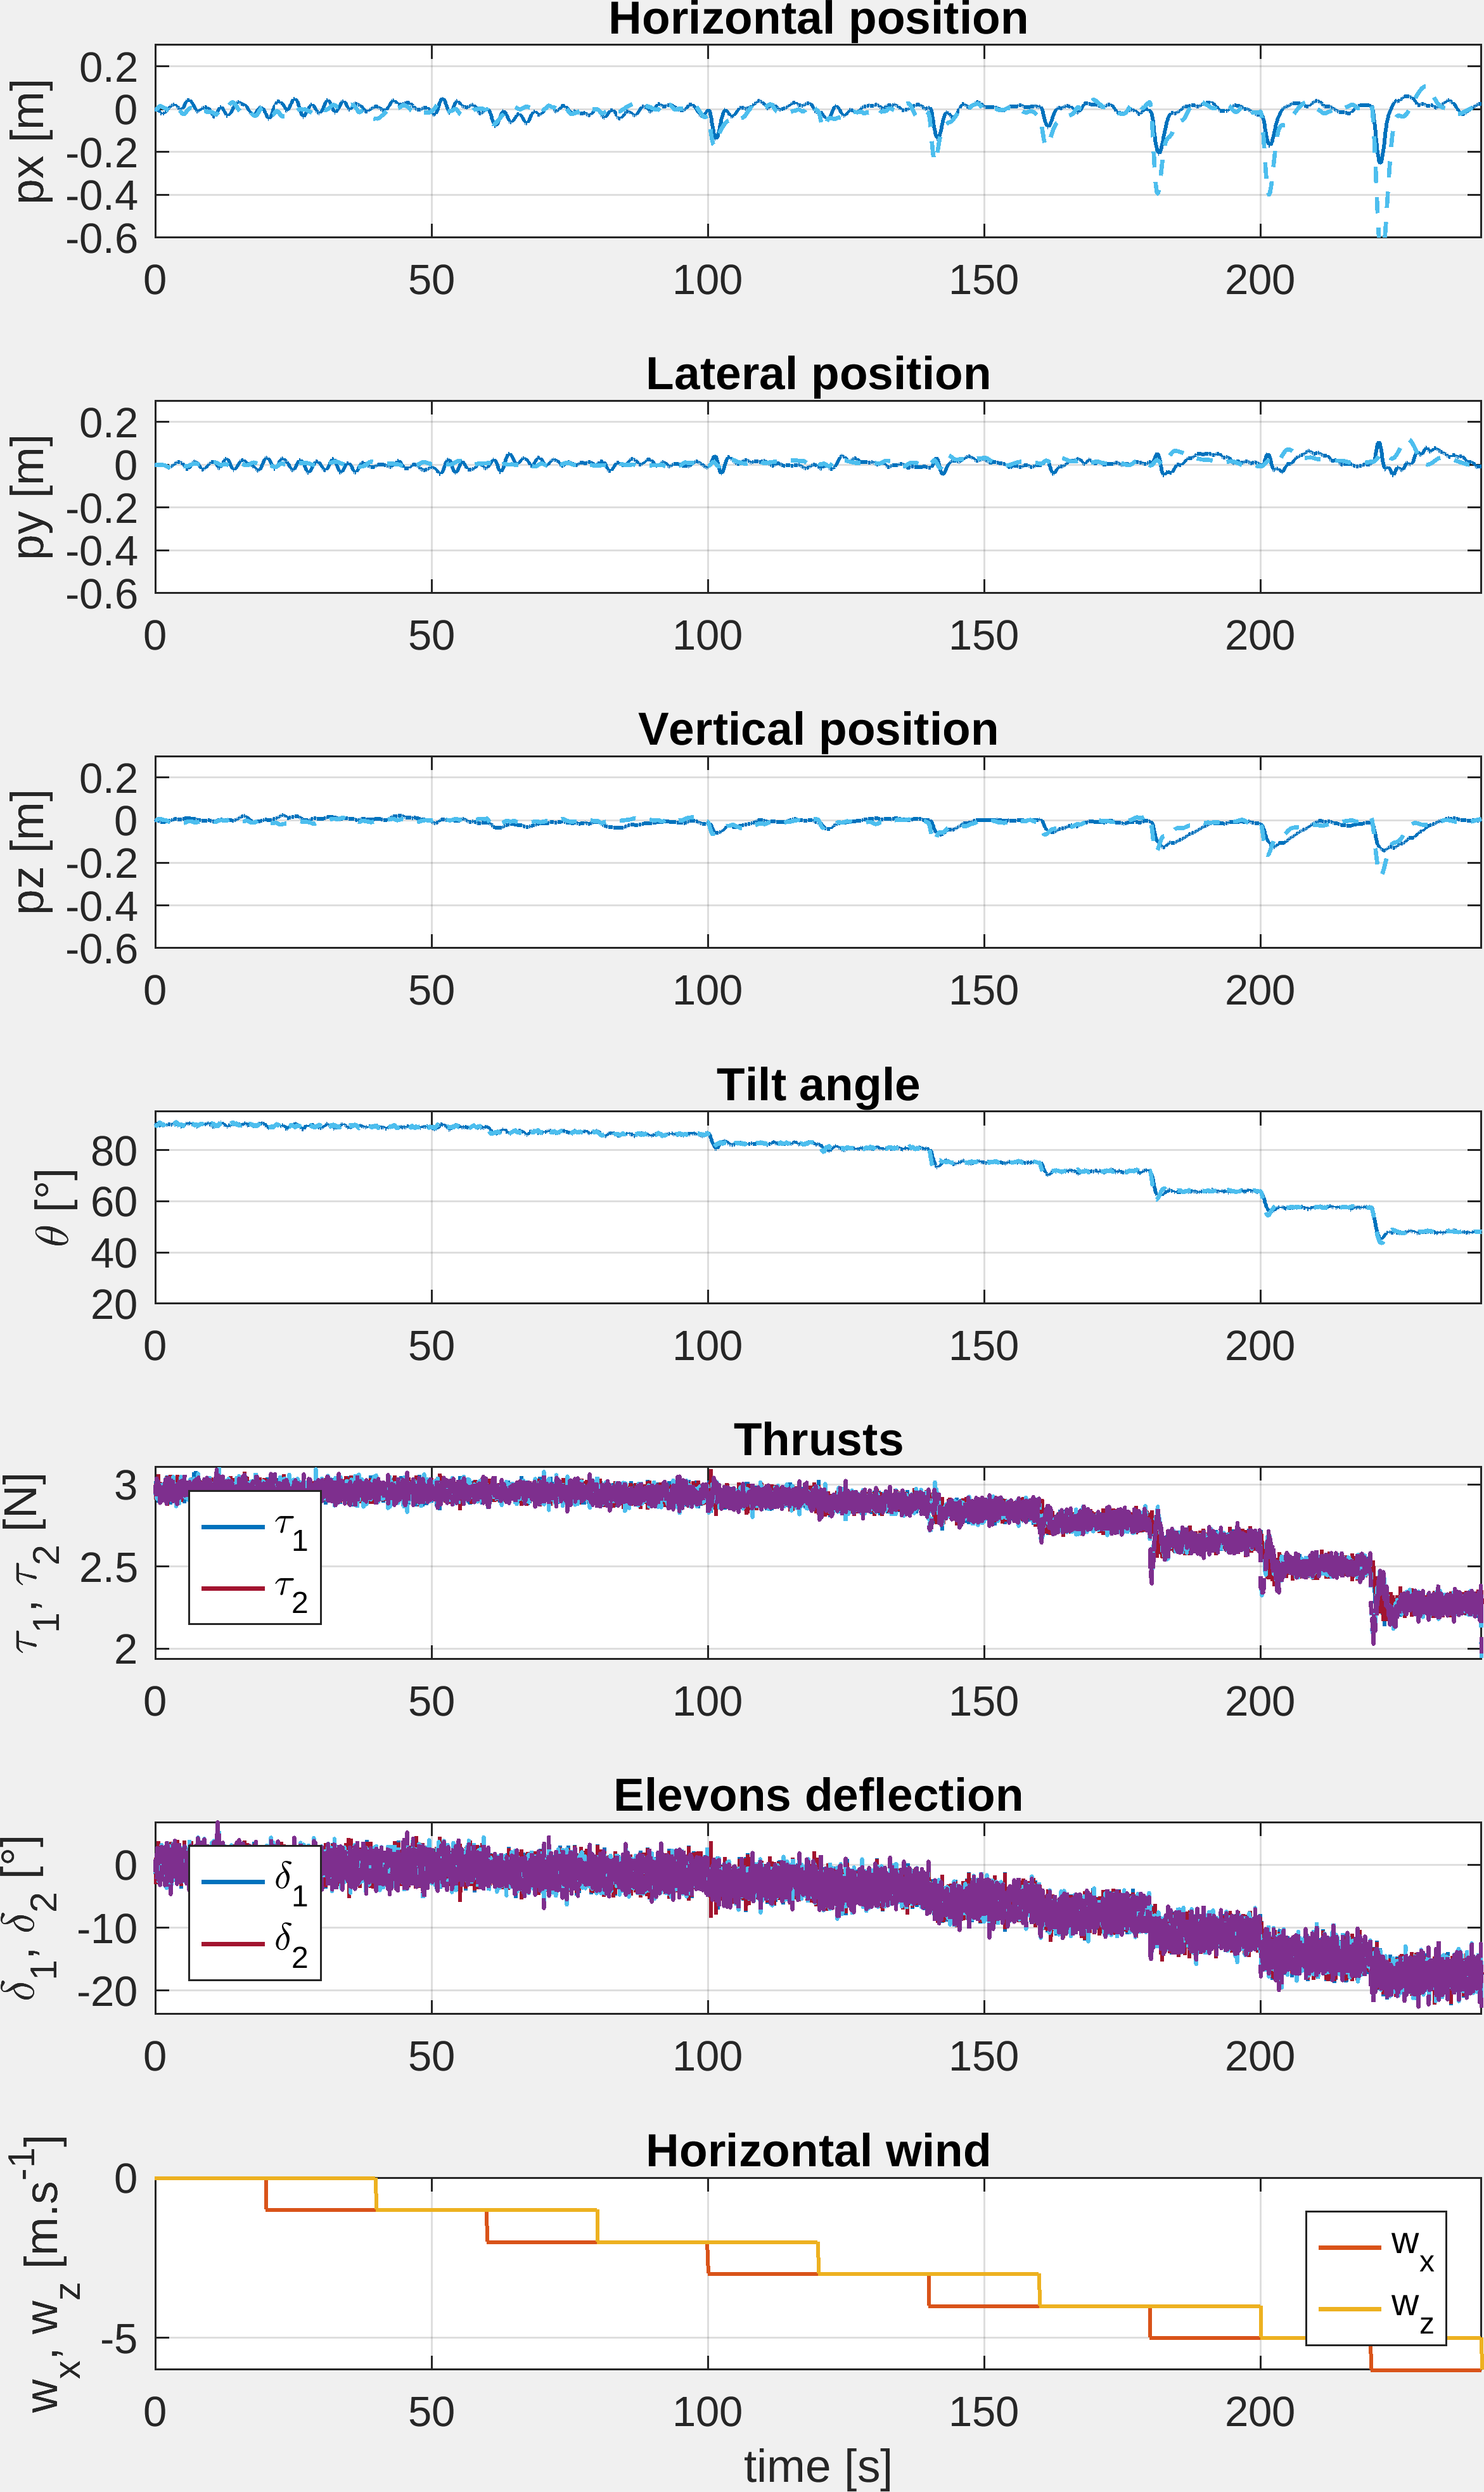
\includegraphics[trim=0cm 0cm 0cm 0cm,clip,width=0.9\columnwidth]{figures/sim_systune_lpv_noise.png}
    \caption{Simulation of the non-linear model \eqref{eq:dyna_orig} (solid line) and the linearized model  \eqref{eq:lpv_linearisation} (dashed line) with increasing constant wind steps with the controller tuned using the multimodel optimization of Algorithm~\ref{alg:iterativeOptimisation} in  Section~\ref{sec:h_inf6DOF_multi}.}
    \label{fig:SimSytuneStruct_lpv}
\end{figure}

With the tuning reported in \eqref{eq:gain_selection}, as obtained with Algorithm~\ref{alg:iterativeOptimisation}, we report in  Fig.~\ref{fig:SimSytuneStruct_lpv} parallel simulation results to those already shown in Fig.~\ref{fig:SimSytuneStruct_zero} for the zero-wind tuning method discussed in Section~\ref{sec:zerowind}. Once again we simulate both the nonlinear plant \eqref{eq:dyna_orig} (solid lines) and the linearized plant \eqref{eq:lpv_linearisation} (dashed line). 
As compared to Fig.~\ref{fig:SimSytuneStruct_zero}, the simulations of Fig.~\ref{fig:SimSytuneStruct_lpv} show that the controller tuning based on Theorems~\ref{thm:eqs} and~\ref{th:lin} 
solves the instability issues and manages to stabilize the hovering condition in all of the considered wind scenarios. We also note from 
Fig.~\ref{fig:SimSytuneStruct_lpv} shows a more aggressive action, indeed the control input $u$ (both thrust and deflections) is more affected by the measurement noise.
The effectiveness of the control scheme tuned on the basis of Algorithm~\ref{alg:iterativeOptimisation} is also confirmed by the experimental results reported in the next section.

% a larger stability range than in the case without wind (Fig.~\ref{fig:SimSytuneStruct_zero}), as we manage to stabilize the drone up to a vertical and horizontal speed of \SI{-6}{\meter\per\second}.


\section{Experimental flight with open wind tunnel} 
\label{sec:exp6DOF}
DarkO's experimental flight took place in a dedicated space (see Fig.~\ref{fig:flight_windshape}) with an Optitrack localization system based on a NED convention as per Figure~\ref{fig:darko2}. We used an open-vein wind generator to obtain wind steps that we measured with a hot-wire probe (the vertical bar in Fig.~\ref{fig:flight_windshape}). 
\begin{figure}[ht!]
    \centering
    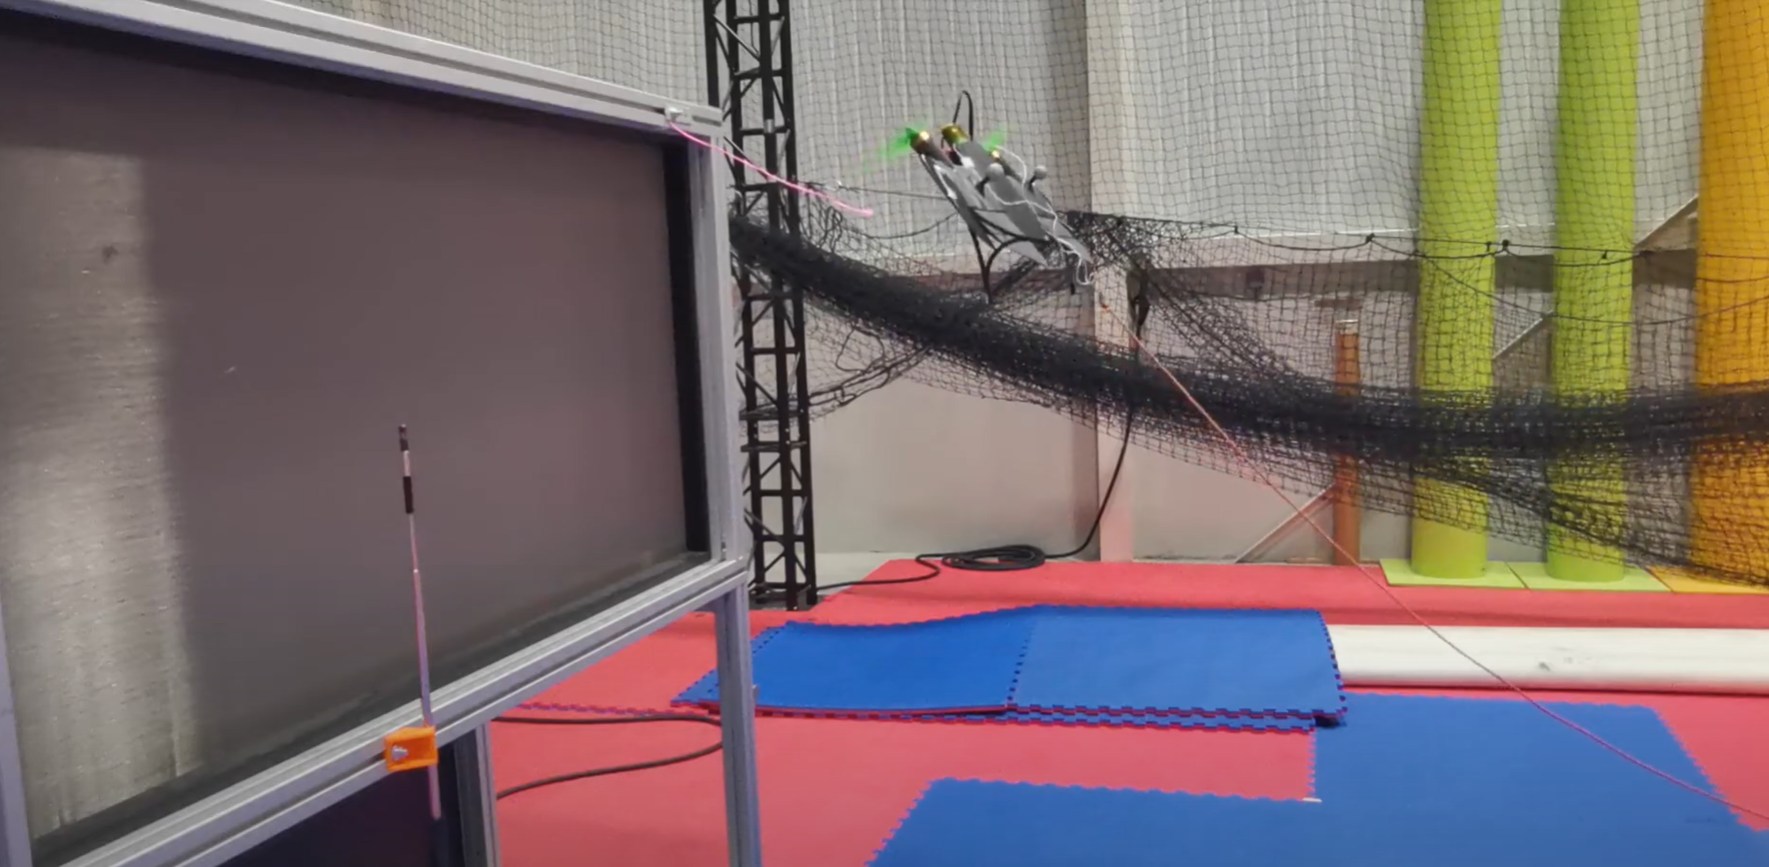
\includegraphics[trim=0cm 0cm 0cm 0cm,clip,width=1\columnwidth]{figures/img_flight_darko.png}
    \caption{DarkO's experimental flight in front of the open wind tunnel.}
    \label{fig:flight_windshape}
\end{figure}
Although this wind information is recorded on board the drone to synchronize the data, we do not use this measurement in the control law. The measurement frequency of this wind probe is only 0.5 Hz, so we only have one measurement every two seconds. 
The state estimation is carried out using an inertial navigation system to merge the Inertial Measurement Unit (IMU) + Optitrack sensor data in order to obtain an accurate estimation of the output $\boldsymbol{y}$ in Fig.~\ref{fig:commande_int6DOF}. However, the drone's angular velocity $\boldsymbol{\omega}_{\text{b}}$ is measured based on the IMU's gyrometer, which provides noisy measurements, therefore we added a second order Butterworth low-pass filter with cut-off frequency of 20 Hz to smoothen out the output $\boldsymbol{\omega}_{\text{b}}$. The Butterworth filter is considered in the linearized dynamics when optimizing the controller gains following Algorithm~\ref{alg:iterativeOptimisation}. 
\todo{comparaison lineaire}
\begin{figure}[ht!]
    \centering
    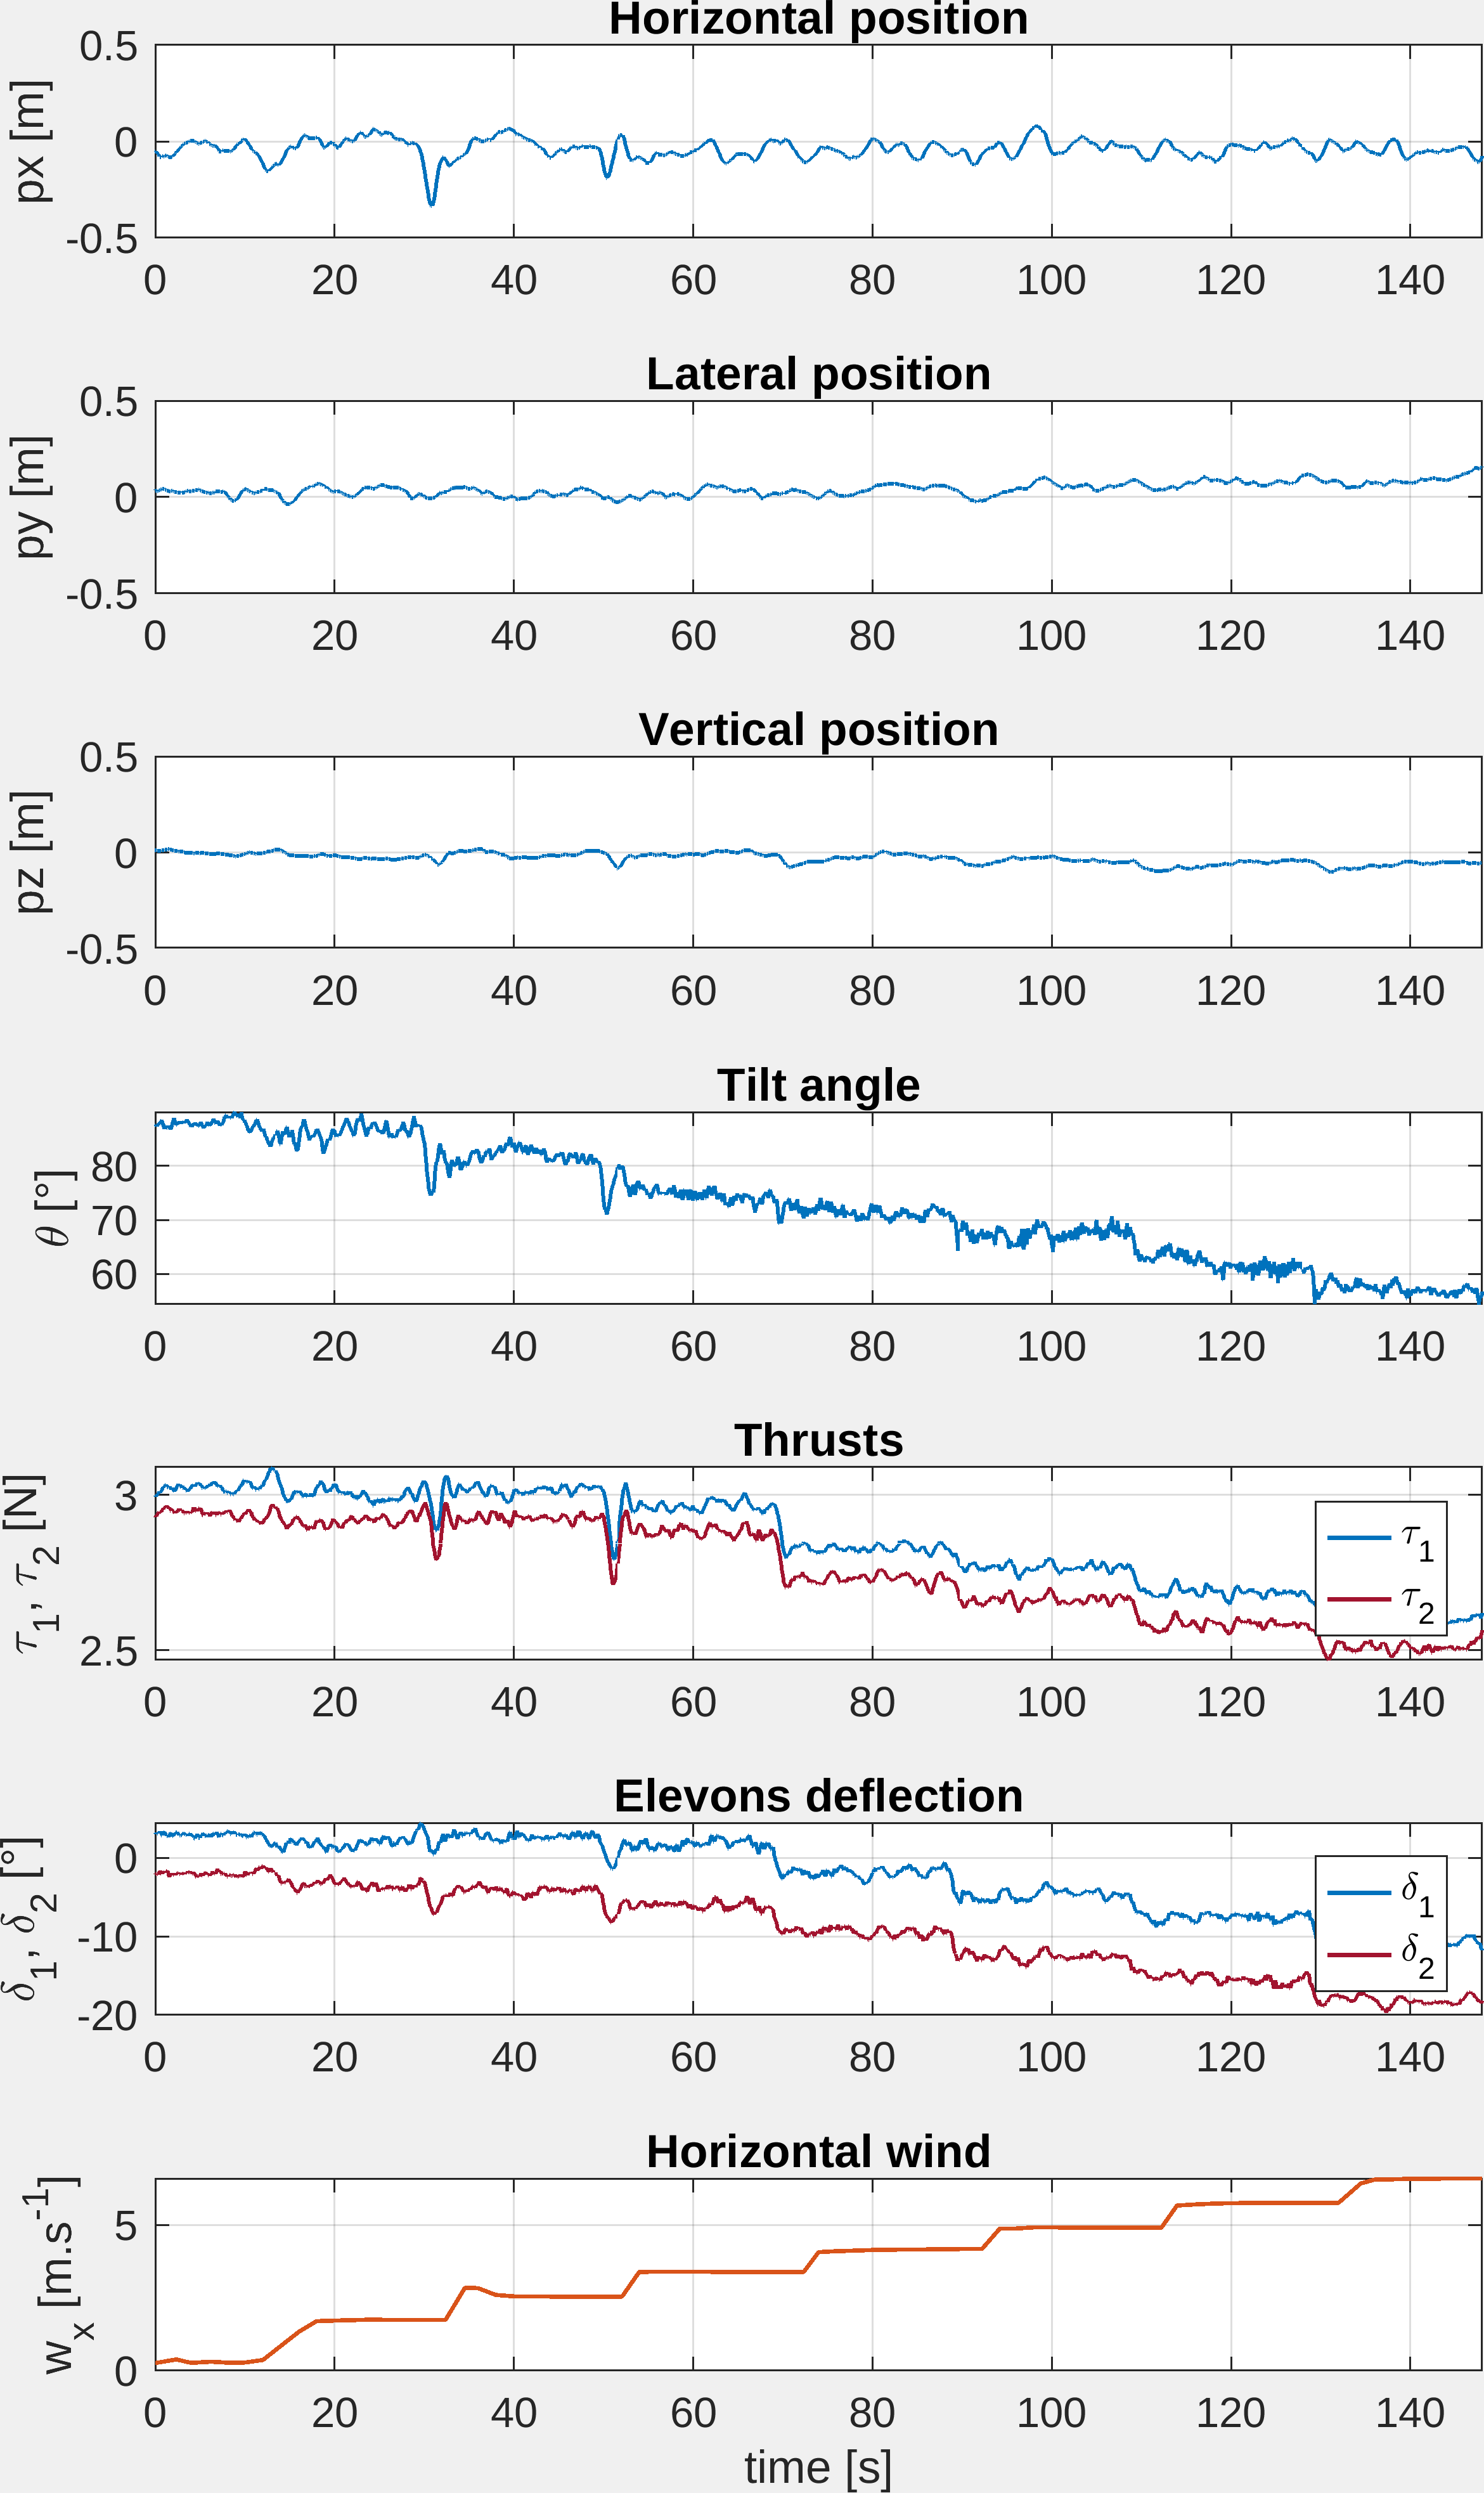
\includegraphics[trim=0cm 0cm 0cm 0cm,clip,width=0.9\columnwidth]{figures/exp_systune_struct.png}
    %'/home/florian/Log/DarkoLog/09_11_23/23_11_05__06_40_06_SD.data'
    \caption{Experiment of the DarkO UAV in front of the wind tunnel with increasing constant wind levels (lower plot).}
    \label{fig:ExpSytuneStruct}
\end{figure}

We also used the ESCs associated with the performance shown in Figure~\ref{fig:IOmot} for the propellers actuation. The two ESCs were flashed with the open-source code available in the GitHub repository AM32-MultiRotor-ESC-firmware\footnote{\url{https://github.com/FlorianSan/AM32-MultiRotor-ESC-firmware}}. The advantage of this firmware, as compared with the commercial code, is that it exploits a low-level PID feedback of the speed of rotation of the motor, which is calculated at the same speed as the motor phase commutation. We adapted the speed loop code in the firmware, following the approach of \cite{franchi2017}, featuring an adaptive bias and adaptive gain algorithm (ABAG). In this way, we compensate the battery discharge effects and obtain an accurate realization of the commanded speed. Before this modification, the integral action of the stabilizing feedback of Fig.~\ref{fig:commande_int6DOF} compensated for the motor speed loss caused by the battery voltage reduction during flight. This integral compensation was indirectly generated by the altitude loss of the UAV caused by the reduced traction. The advantages of the ABAG solution are high responsiveness and adaptability, as the propeller dimensions can be changed without needing to modify the actuation gains.

We carried out a flight experiment where DarkO was manually put into a stabilized hovering mode in front of the wind tunnel, then we switched on the control law of Algorithm~\ref{alg:iterativeOptimisation}. As the drone had to be stabilized at least \SI{30}{\centi\meter} away from the wind tunnel, a manual command was gradually applied to avoid overshooting, which could damage the wind tunnel. Once DarkO was close enough to the setpoint $\boldsymbol{r}_{p}$ of Fig.~\ref{fig:commande_int6DOF}, we switched on the proposed controller, obtaining the results in Fig.~\ref{fig:ExpSytuneStruct}. During the follow-up experimentation phase, as shown in the lower plot of Fig.~\ref{fig:ExpSytuneStruct}, we stepwise increased the wind speed, waiting 20 seconds between each  pair of consecutive steps, up to a final wind speed of \SI{7}{\meter\per\second}.

\begin{figure}[ht!]
    \centering
    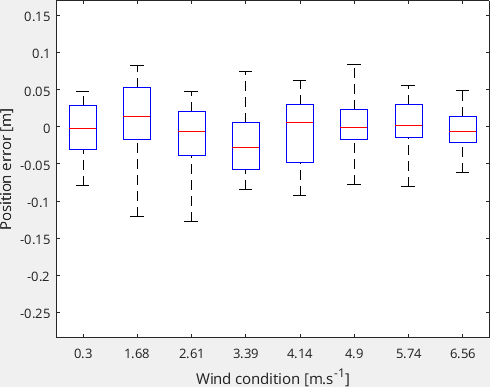
\includegraphics[trim=0cm 0cm 0cm 0cm,clip,width=0.9\columnwidth]{figures/boxplot.png}
    \caption{Statistical visualization of the hovering performance.}
    \label{fig:statpos}
\end{figure}
Figs~\ref{fig:ExpSytuneStruct} and~\ref{fig:statpos} show that the drone maintains its position despite the increasing wind speed. We can note a few important points, in agreement with the simulations: the motor traction decreases when increasing the wind speed. The control scheme takes advantage of the lift generated by the wind to support the drone, so that less energy is needed to stabilize the hovering position. The drone maintains its tilt angle at a value that is unknown a priori to the control law and naturally stems from the integral action that asymptotically attains the required value of the drone's pitch angle $\theta$. To stabilize the position, the UAV uses the elevons to cancel the pitch moment generated by the shape of the wing, subjected to a horizontal wind, without reaching the saturation limits.
We also notice a slight asymmetry of the effectiveness of the actuators, which is effectively compensated by the proportional action of the control scheme.
\section{Maquette expérimentale : 6 Dof}

\section{Résultats}

\section{Conclusion du Chapitre \ref{chap:6DOF}}




